\documentclass[11pt]{article}

\usepackage[margin=1in]{geometry}
\usepackage[T1]{fontenc}
\usepackage[utf8]{inputenc}
\usepackage{microtype}
\usepackage{setspace}
\usepackage{booktabs}
\usepackage{longtable}
\usepackage{array}
\usepackage{hyperref}
\usepackage{tikz}
\usepackage[numbers,sort&compress]{natbib}

\title{Workplace Determinants of Metabolic Syndrome in Working Adults: Systematic Review}
\author{}
\date{}

\begin{document}
\maketitle

\section*{Teaser text}
Workplace stress, unhealthy dietary patterns, physical inactivity and prolonged sedentary behaviour are associated with metabolic syndrome among working adults. Prospective and intervention studies also indicate that workplace-based programmes targeting diet, activity and broader lifestyle factors can improve metabolic outcomes, supporting the workplace as an important setting for cardiometabolic prevention.

\begin{abstract}
\textbf{Background:}
Metabolic syndrome (MetS) is influenced by occupational and behavioural factors that cluster within working populations, while workplaces also provide a practical setting for prevention.

\textbf{Aims:}
To synthesize evidence on workplace stress, diet, physical activity, sedentary behaviour, and MetS among working adults, and to evaluate workplace-based lifestyle interventions targeting MetS or its components.

\textbf{Methods:}
Peer-reviewed studies published from 2015 to 2026 were identified using a workplace-focused search. Eligible studies examined employed adults or occupational populations and evaluated relevant exposures or workplace lifestyle interventions in relation to MetS or established components. Randomized trials, cohort studies, analytical cross-sectional studies, and quasi-experimental interventions were eligible. Design-specific Joanna Briggs Institute tools were used for critical appraisal. Heterogeneous evidence was synthesized narratively.

\textbf{Results:}
Prospective evidence generally linked adverse work stress with greater MetS risk. Higher leisure-time physical activity was associated with lower MetS incidence or prevalence, whereas prolonged sedentary exposure was associated with greater risk. Healthier dietary patterns were generally associated with more favourable metabolic profiles. Workplace interventions involving exercise, dietary modification, counselling, or multicomponent lifestyle support improved waist circumference, blood pressure, glucose regulation, lipid profiles, or MetS severity in several studies. Observational evidence was heterogeneous and frequently cross-sectional.

\textbf{Conclusions:}
Workplace stress, diet, physical activity, and sedentary behaviour are important modifiable correlates of MetS among working adults. Workplace lifestyle interventions can improve metabolic outcomes, although confidence is greatest for randomized and prospective evidence.

\textbf{Keywords:} metabolic syndrome; occupational stress; workplace; diet; physical activity; sedentary behaviour; occupational health; systematic review
\end{abstract}

\section{Introduction}

Metabolic syndrome (MetS) is a clustering of cardiometabolic abnormalities that commonly includes central obesity, elevated blood pressure, impaired glucose regulation, hypertriglyceridaemia, and reduced high-density lipoprotein cholesterol. Its clinical importance lies in the increased risk of type 2 diabetes and cardiovascular disease associated with accumulation of these abnormalities.

For working adults, MetS is especially relevant because many of its determinants are shaped by the conditions in which people work. Sedentary occupations can reduce daily energy expenditure, irregular or extended working hours may disrupt eating patterns and recovery, and high psychosocial demands may reinforce behaviours such as physical inactivity and unhealthy food choices. Occupational stress may also influence metabolic risk through prolonged physiological activation.

Evidence from occupational populations supports this concern. Prospective studies of police officers and manufacturing workers have linked higher or increasing work stress with subsequent MetS risk \citep{Garbarino2015,Yamaguchi2018}. Large workforce cohorts have demonstrated differences in MetS incidence across occupational groups \citep{vanZon2020Occupational,Runge2021Metabolic}. Physical activity also appears relevant, with prospective worker studies suggesting lower MetS incidence among those engaging in greater leisure-time exercise \citep{Kuwahara2016}, whereas prolonged sedentary exposure has been associated with higher MetS prevalence \citep{Motuma2020}. Workplace dietary patterns and nutrition interventions provide a further modifiable pathway \citep{Kim2016Dietary,Ma2025}.

Workplaces therefore represent both a source of metabolic risk and a practical setting for prevention. Randomized and quasi-experimental studies have evaluated exercise, dietary modification, digital health support, counselling, self-monitoring, and multicomponent lifestyle programmes \citep{Haufe2019,Choi2017,Ryu2017,So2025,Bogale2025}.

Despite this growing literature, the evidence remains fragmented. Studies differ substantially in occupational populations, exposure definitions, intervention intensity, MetS criteria, outcome reporting, and methodological design. A focused synthesis of workplace evidence is therefore needed.

The aim of this systematic review was to synthesize evidence on the relationships between workplace stress, dietary factors, physical activity, sedentary behaviour, and MetS among working adults. A secondary aim was to evaluate the effectiveness of workplace-based lifestyle interventions targeting MetS or its established metabolic components.

\section{Methods}

\subsection{Design and reporting framework}

This systematic review was updated and restructured to evaluate the relationships between workplace stress, dietary factors, physical activity, and MetS among working adults. The review used a workplace-focused eligibility framework and followed PRISMA principles.

The original undergraduate thesis served as the historical starting point. Because the original screening spreadsheet was unavailable and the archived thesis study set contained eligibility inconsistencies, a fresh literature search and re-screening process were undertaken for the revised manuscript.

\subsection{Eligibility criteria}

Participants were adults in employment, occupational groups, or explicitly defined workplace settings. Eligible exposures or interventions included occupational stress, job strain, dietary patterns, diet quality, nutrition, workplace food interventions, physical activity, exercise, sedentary behaviour, work-related activity, and multicomponent workplace lifestyle interventions.

Studies were required to report MetS as a defined syndrome or recognized MetS components explicitly framed in relation to MetS prevention, risk, severity, or management. Recognized components included central or abdominal obesity, elevated blood pressure, impaired fasting glucose or hyperglycaemia, elevated triglycerides, and reduced HDL cholesterol.

Completed original empirical studies were eligible, including randomized controlled trials, prospective or longitudinal cohort studies, analytical cross-sectional studies, and quasi-experimental workplace interventions. Study protocols, editorials, conference abstracts, grey literature, and secondary reviews were excluded from the primary evidence synthesis. English-language peer-reviewed studies published from 2015 through 2026 were eligible.

\subsection{Search strategy}

The primary search concepts combined terms for MetS, workers or workplaces, and workplace stress, physical activity, sedentary behaviour, diet, nutrition, and lifestyle intervention. PubMed/MEDLINE was the primary bibliographic source. Supplementary searches used narrower exposure-specific combinations, and additional studies were identified through reference-list screening, citation chasing, publisher records, PubMed related-article searching, and review-article reference mining.

The final database-specific search strings, exact search dates, and record counts are maintained in the repository search log. Final PRISMA counts remain to be frozen after complete export and deduplication.

\subsection{Study selection and data extraction}

Screening was performed in two stages: title/abstract screening followed by full-text eligibility assessment. Where multiple publications arose from the same underlying cohort or intervention programme, the reports were linked and treated as companion publications rather than independent populations when participant totals or evidence weight were summarized.

A structured extraction table captured author, year, country, occupational population, design, sample size, follow-up, exposure or intervention, MetS definition or outcome, principal effect estimates, methodological limitations, and bibliographic identifier. Adjusted estimates were preferred where available, and between-group effects were prioritized for intervention studies.

\subsection{Critical appraisal}

Methodological quality was assessed using design-specific Joanna Briggs Institute tools for randomized controlled trials, cohort studies, analytical cross-sectional studies, and quasi-experimental studies. Items were judged as Yes, No, Unclear, or Not applicable where permitted. Studies were not excluded solely on the basis of a numerical appraisal score.

\subsection{Data synthesis}

Because of substantial heterogeneity in occupational populations, exposure definitions, intervention content, MetS definitions, study designs, and effect measures, the primary synthesis was narrative. Evidence was organized into occupational stress, diet and workplace nutrition, physical activity and sedentary behaviour, and multicomponent workplace lifestyle interventions. Interpretation prioritized randomized trials, followed by prospective cohort studies, quasi-experimental studies, and analytical cross-sectional studies.

\section{Results}

\subsection{Study selection and characteristics}

The current active evidence pool contains 34 primary studies published between 2015 and 2026. Because database export and deduplication are still being finalized, this number should not yet be treated as the definitive PRISMA included-study count.

The evidence base comprised randomized controlled trials, prospective cohort studies, analytical cross-sectional studies, and quasi-experimental workplace interventions. Occupational populations included office and white-collar workers, police and security personnel, commercial and tanker drivers, manufacturing and petrochemical workers, healthcare professionals, university staff, military personnel, heavy-industry workers, and employees enrolled in workplace health-promotion programmes.

\section*{Table 1. Characteristics of the active study pool}

\begin{longtable}{p{0.16\textwidth} p{0.25\textwidth} p{0.20\textwidth} p{0.29\textwidth}}
\toprule
Study & Occupational population & Design & Main exposure/intervention \\
\midrule
\endfirsthead
\toprule
Study & Occupational population & Design & Main exposure/intervention \\
\midrule
\endhead
    Alavi (2015) & Office workers & Analytical cross-sectional & Lifestyle/occupational factors \\
    Garbarino (2015) & Police officers & Prospective cohort & Work stress \\
    Kuwahara (2016) & Japanese workers & Prospective cohort & Physical activity \\
    Ko (2016) & Male public-office workers & Analytical cross-sectional & Physical activity \\
    Browne et al. (2017) & Sedentary occupation workers & Analytical cross-sectional & Physical activity \\
    Yamaguchi (2018) & Japanese manufacturing workers & Prospective cohort & Work-related stress \\
    Haufe (2019) & Volkswagen company employees & Randomized controlled trial & Exercise \\
    Appiah (2020) & Commercial taxi drivers & Analytical cross-sectional & Diet/lifestyle/physical inactivity \\
    Aboma (2020) & Working adults & Analytical cross-sectional & Lifestyle/diet/sedentary behaviour \\
    Jovanovic et al. (2020) & Security guards & Analytical cross-sectional & Occupational stress \\
    van Zon et al. (2020) & Dutch workers across occupational groups & Cohort/longitudinal observational & Occupation/physical activity/diet \\
    van Zon et al. (2021) & Older workers & Prospective cohort & Diet/physical activity/health behaviours \\
    Eftekhari (2021) & Medical university staff & Analytical cross-sectional & Job stress \\
    Apprey (2022) & Fuel tanker drivers & Analytical cross-sectional & Dietary intake \\
    Zhang (2024) & Petrochemical workers & Analytical cross-sectional & Occupational stress \\
    Sharifi (2025) & Health workers & Analytical cross-sectional & Diet quality \\
    Ma (2025) & Occupational men at oilfield canteens & Randomized controlled trial & Dietary intervention \\
    dos Reis et al. (2026) & Healthcare workers & Analytical cross-sectional & Night work/diet \\
    Petek \& Karabudak (2026) & Heavy-industry workers & Analytical cross-sectional & Diet/nutritional status \\
    Reinoso-Barbero et al. (2026) & Multinational-company employees & Analytical cross-sectional & Mediterranean diet \\
    Ayeltigah et al. (healthcare) (2026) & Healthcare professionals & Analytical cross-sectional & Stress/diet/physical activity \\
    Ayeltigah et al. (university) (2026) & University workers & Analytical cross-sectional & Stress/diet/physical activity \\
    Ayeltigah et al. (military) (2026) & Military personnel & Analytical cross-sectional & Work stress/diet/physical activity \\
    Earnest (2015) & Employees from 93 companies & Quasi-experimental pre-post & Worksite behavioral weight-loss intervention \\
    Kim et al. (2016) & Male white-collar employees & Quasi-experimental pre-post & Dietary intervention and worksite food environment \\
    Ryu (2017) & Office workers & Quasi-experimental pre-post & Workplace health promotion: education/self-monitoring/diet/activity \\
    So (2025) & Employees & Quasi-experimental single-group longitudinal & HIIT plus calorie restriction \\
    Bogale (2025) & Bank employees/office workers & Randomized controlled trial & Lifestyle education: diet/physical activity/stress and other risk factors \\
    Kim et al. BEST (2015) & Korean male workers with MetS & Controlled nonrandomized trial & Physical activity/diet/counselling \\
    Choi (2017) & Middle-aged male office workers & Randomized controlled trial & T'ai Chi + health education \\
    Huang et al. (2017) & Taiwanese workers & Analytical cross-sectional & Occupational/leisure/commuting physical activity \\
    Fang et al. (2019) & Overweight sedentary high-tech employees & Randomized controlled trial & Physical activity program \\
    Schilling et al. (2020) & Police officers & Prospective cohort & Work stress/physical activity/cardiorespiratory fitness \\
    Park \& Hwang (2024) & Male office workers with MetS & Randomized controlled trial & Remote physical activity program \\
\bottomrule
\end{longtable}

\noindent\textit{Note:} The active pool currently contains 34 primary studies. Final PRISMA study/report counts remain provisional pending complete search export and deduplication.

\section*{Table 2. Principal findings from higher-priority and quantitatively informative studies}

\begin{longtable}{p{0.15\textwidth} p{0.20\textwidth} p{0.31\textwidth} p{0.27\textwidth}}
\toprule
Study & Domain & Key result & Interpretation \\
\midrule
\endfirsthead
\toprule
Study & Domain & Key result & Interpretation \\
\midrule
\endhead
    Garbarino (2015) & Work stress & aOR 2.68 (95\% CI 1.08-6.70) & Higher work stress predicted incident MetS \\
    Kuwahara (2016) & Physical activity & HR 0.74 (95\% CI 0.62-0.89) for 7.5 to <16.5 MET-h/week; HR 0.81 (0.69-0.96) for $\geq$16.5 & Higher-intensity mixed leisure exercise associated with lower MetS incidence; commuting walking not associated \\
    Browne et al. (2017) & Physical activity & Active vs sedentary: MetS OR 0.52 (95\% CI 0.27-0.98); abdominal obesity OR 0.36 (0.16-0.82); elevated BP OR 0.47 (0.26-0.84); low HDL OR 0.54 (0.31-0.93) & Meeting PA recommendations was associated with lower MetS and component risk \\
    Yamaguchi (2018) & Work-related stress & aOR 3.27 (95\% CI 1.46-7.34) & Increasing job demands over time associated with higher incident MetS \\
    Haufe (2019) & Exercise & Between-group difference -0.26 (95\% CI -0.35 to -0.16); p<0.0001 & Telemonitoring-supported exercise reduced MetS severity \\
    Aboma (2020) & Lifestyle/diet/sedentary behaviour & Sedentary $\geq$8 h: APR 2.29 (95\% CI 1.88-2.80); $\geq$5 fruit/veg servings: APR 0.04 (0.01-0.27) & Sedentary time associated with higher MetS prevalence; high fruit/vegetable intake with lower prevalence \\
    van Zon et al. (2020) & Occupation/physical activity/diet & Men stationary plant/machine operators HR 1.94 (95\% CI 1.26-3.00); women food-preparation assistants HR 1.80 (1.01-3.22) & MetS risk differed by occupation and sex \\
    van Zon et al. (2021) & Diet/physical activity/health behaviours & Low-skilled white-collar OR 1.24 (95\% CI 1.12-1.37); low-skilled blue-collar OR 1.37 (1.18-1.59) & Older low-skilled workers had higher incident MetS; behaviours explained part of differences \\
    Eftekhari (2021) & Job stress & Office workers OR 1.51 (95\% CI 1.25-1.82); service personnel OR 1.74 (1.41-2.14) vs clinical staff & MetS prevalence varied by employment category; psychosocial well-being was poorer with MetS \\
    Zhang (2024) & Occupational stress & No overall association with MetS; adjusted models linked D/C ratio with SBP, social support with waist circumference, and over-commitment with fasting blood glucose & Occupational stress was not associated with MetS overall, but selected stress dimensions were associated with specific MetS components \\
    Sharifi (2025) & Diet quality & MetS prevalence 22.3\%; diet moderation associated with MetS OR 1.03 (95\% CI 1.008-1.05), abdominal obesity OR 1.02 (1.003-1.04), elevated TG OR 1.02 (1.00-1.03), elevated FBS OR 1.03 (1.005-1.05) & Diet moderation score was associated with MetS and several components; adequacy was not \\
    Ma (2025) & Dietary intervention & FBG beta -0.72 p=0.010; TC -1.49 p<0.001; LDL-C -0.65 p<0.001; WC -7.73 p<0.001; BMI -2.01 p<0.001; HDL-C +0.13 p<0.001 & Canteen-based healthy lunch plus advice improved several MetS components \\
    Ayeltigah et al. (military) (2026) & Work stress/diet/physical activity & Work stress and MetS: OR 6.472 (95\% CI 1.535-27.292) & Work stress associated with higher MetS odds; estimate imprecise \\
    Earnest (2015) & Worksite behavioral weight-loss intervention & Women 43\% to 30\%; men 52\% to 26\%; p<0.001 & Voluntary worksite weight-loss program reduced MetS prevalence and risk factors \\
    Ryu (2017) & Workplace health promotion: education/self-monitoring/diet/activity & Targeted intensive group: waist 89.96 to 86.93 cm and fasting glucose 93.44 to 84.56 mg/dL, p<0.001; MetS prevalence 41.5\% to 31.7\% & Targeted proactive workplace program improved MetS indicators; voluntary low-intensity components did not \\
    So (2025) & HIIT plus calorie restriction & Weight, blood pressure and triglycerides improved post-intervention and remained improved at 1 year (p<0.01) & Web-based HIIT + calorie restriction improved MetS-related outcomes \\
    Bogale (2025) & Lifestyle education: diet/physical activity/stress and other risk factors & Waist -5.33 cm; SBP -6.96 mmHg; DBP -4.21 mmHg; total cholesterol -34.12 mg/dL; LDL -20.68 mg/dL; all p<0.0001 & Workplace lifestyle education improved several MetS risk factors \\
    Kim et al. BEST (2015) & Physical activity/diet/counselling & Weight p=0.022; visceral fat p=0.033; waist circumference p=0.037 & Internet-based activity/diet/counselling improved selected cardiometabolic risks \\
    Choi (2017) & T'ai Chi + health education & SBP p=0.003; DBP p=0.037; triglycerides p=0.019 & T'ai Chi plus health education improved blood pressure and triglycerides \\
    Huang et al. (2017) & Occupational/leisure/commuting physical activity & High vs low leisure-time PA: OR 0.76 (95\% CI 0.62-0.95) & Higher leisure-time PA associated with lower MetS odds; commuting PA not associated \\
    Fang et al. (2019) & Physical activity program & Reduced number of MetS risk factors; lower triglycerides, total cholesterol and LDL & Worksite PA program improved metabolic and fitness outcomes \\
    Schilling et al. (2020) & Work stress/physical activity/cardiorespiratory fitness & Cardiorespiratory fitness predicting MetS risk: beta -0.38 & Higher fitness predicted lower follow-up MetS risk; no main effect for PA or work stress \\
    Park \& Hwang (2024) & Remote physical activity program & Intervention improved physical and physiological indicators versus control (P<0.05) & Remote workplace PA education improved MetS-related indicators \\
\bottomrule
\end{longtable}

\noindent\textit{Abbreviations:} APR, adjusted prevalence ratio; aOR, adjusted odds ratio; BMI, body mass index; CI, confidence interval; FBG, fasting blood glucose; HDL, high-density lipoprotein; HR, hazard ratio; LDL, low-density lipoprotein; MetS, metabolic syndrome; OR, odds ratio; PA, physical activity; SBP, systolic blood pressure; WC, waist circumference.

\section*{Table 3. Provisional methodological appraisal summary}

\begin{tabular}{p{0.24\textwidth} p{0.07\textwidth} p{0.18\textwidth} p{0.43\textwidth}}
\toprule
Design group & n & JBI tool & Main appraisal pattern \\
\midrule
    Randomized controlled trials & 6 & JBI RCT & Randomized comparisons strengthen causal inference, but concealment, masking, attrition and analysis by randomized assignment remain incompletely reported in some trials. \\
    Prospective/cohort studies & 6 & JBI Cohort & Generally stronger temporal ordering; attrition and missing-data handling are the main recurring uncertainties, and one police study did not require MetS absence at baseline. \\
    Analytical cross-sectional studies & 17 & JBI analytical cross-sectional & Useful for occupational associations but unable to establish temporality; reverse causation remains possible. \\
    Quasi-/nonrandomized interventions & 5 & JBI quasi-experimental & Useful intervention evidence but weaker causal confidence where randomization, repeated measurements, or concurrent controls are absent. \\
\bottomrule
\end{tabular}

\noindent\textit{Note:} All studies in the active pool have now undergone preliminary design-appropriate appraisal. No arbitrary summed quality score is used; appraisal findings qualify confidence in the narrative synthesis.


\subsection{Occupational and work-related stress}

Prospective evidence supported an association between adverse work stress and subsequent MetS risk. In police officers, high work stress was associated with increased odds of incident MetS over five years (adjusted OR 2.68, 95\% CI 1.08--6.70) \citep{Garbarino2015}. In manufacturing workers, increasing job demands were associated with higher odds of developing MetS over three years (adjusted OR 3.27, 95\% CI 1.46--7.34) \citep{Yamaguchi2018}.

Cross-sectional studies generally pointed in the same direction. Among security guards, higher occupational stressors were associated with adverse glucose, lipid, blood-pressure, and cardiovascular-risk profiles \citep{Jovanovic2020}. In petrochemical workers, occupational stress assessed using job-content and effort--reward imbalance frameworks was associated with MetS and selected components \citep{Zhang2024}. Among Ghanaian military personnel, work stress was associated with higher odds of MetS \citep{Ayeltigah2026Military}.

\subsection{Diet and workplace nutrition}

Dietary evidence included observational studies and workplace interventions. In office workers, lower fruit intake and lower leisure-time physical activity were associated with MetS \citep{Alavi2015}. Among Iranian health workers, diet moderation was associated with MetS and several components \citep{Sharifi2025}. Among workers at a multinational company in Madrid, greater adherence to the Mediterranean diet was associated with lower odds of MetS \citep{ReinosoBarbero2026}.

Intervention evidence was also supportive. A randomized canteen-based dietary intervention improved fasting glucose, total cholesterol, LDL cholesterol, HDL cholesterol, waist circumference, and body mass index \citep{Ma2025}. A Korean worksite dietary intervention likewise reported improvement in MetS indicators following structured dietary modification \citep{Kim2016Dietary}.

\subsection{Physical activity and sedentary behaviour}

Physical activity showed one of the most consistent associations with metabolic health. In a prospective cohort of 22,383 workers, greater leisure-time exercise was associated with lower MetS incidence \citep{Kuwahara2016}. Among sedentary occupation workers, meeting physical-activity recommendations was associated with lower odds of MetS and several MetS components \citep{Browne2017}. In Taiwanese workers, higher leisure-time physical activity was associated with lower MetS odds \citep{Huang2017Taiwan}.

Among working adults in Ethiopia, prolonged sedentary time was associated with substantially higher MetS prevalence \citep{Motuma2020}. Randomized exercise studies reinforced the observational findings. Telemonitoring-supported exercise reduced MetS severity among company employees \citep{Haufe2019}. Workplace T'ai Chi and other structured physical-activity programmes improved selected metabolic outcomes \citep{Choi2017,Fang2019}.

\subsection{Multicomponent workplace lifestyle interventions}

Several studies evaluated interventions combining physical activity, dietary modification, counselling, self-monitoring, or digital support. A voluntary worksite weight-loss programme reduced MetS prevalence in participating employees \citep{Earnest2015}. A targeted workplace health-promotion programme improved waist circumference, fasting glucose, and MetS prevalence \citep{Ryu2017}. An internet-based lifestyle programme improved selected cardiometabolic risk factors \citep{Kim2015Internet}. A web-based high-intensity interval-training plus calorie-restriction programme also improved several MetS-related outcomes \citep{So2025}.

The strongest recent evidence came from randomized programmes. A cluster-randomized lifestyle-education intervention among Ethiopian bank employees reduced waist circumference, blood pressure, and lipid measures \citep{Bogale2025}.

\subsection{Summary of evidence consistency}

Across designs, the evidence generally converged on three patterns. Adverse occupational stress was associated with greater MetS risk, with prospective studies providing the strongest temporal support. Healthier dietary patterns and workplace dietary interventions were associated with more favourable metabolic profiles. Greater physical activity and lower sedentary exposure were consistently associated with reduced MetS risk, and workplace exercise interventions improved several metabolic outcomes.

\begin{figure}[htbp]
\centering
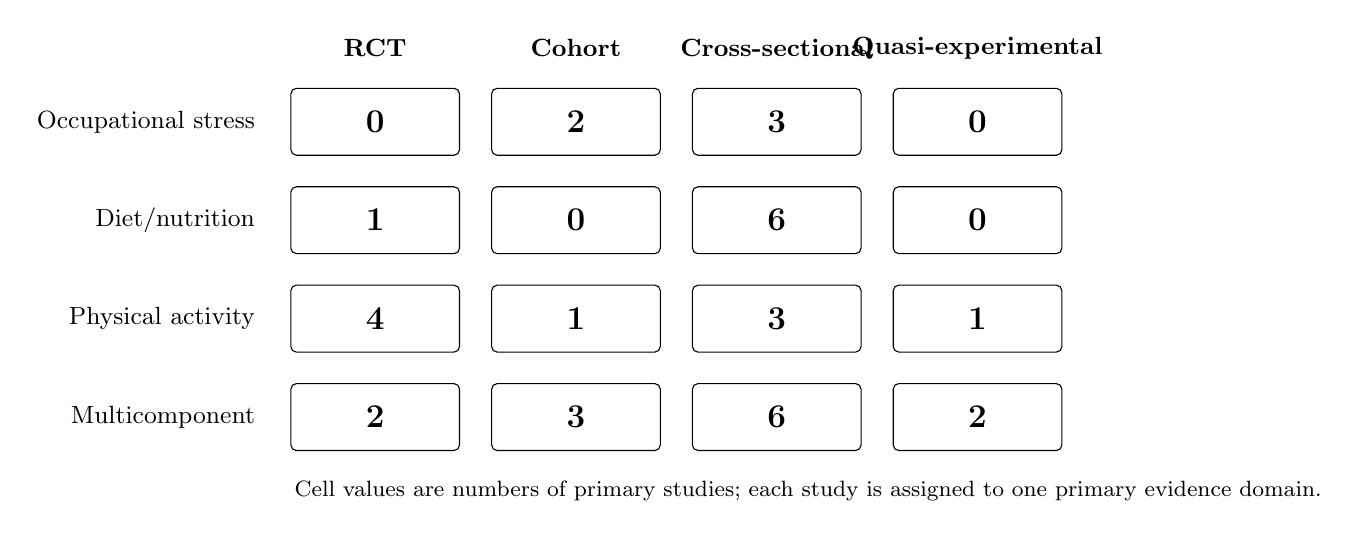
\begin{tikzpicture}[x=2.55cm,y=1.25cm]
  % Column labels
  \node[font=\small\bfseries] at (1,4.75) {RCT};
  \node[font=\small\bfseries] at (2,4.75) {Cohort};
  \node[font=\small\bfseries] at (3,4.75) {Cross-sectional};
  \node[font=\small\bfseries] at (4,4.75) {Quasi-experimental};

  % Row labels
  \node[anchor=east,font=\small] at (0.45,4) {Occupational stress};
  \node[anchor=east,font=\small] at (0.45,3) {Diet/nutrition};
  \node[anchor=east,font=\small] at (0.45,2) {Physical activity};
  \node[anchor=east,font=\small] at (0.45,1) {Multicomponent};

  % Matrix cells
  \foreach \x/\y/\n in {
    1/4/0,2/4/2,3/4/3,4/4/0,
    1/3/1,2/3/0,3/3/6,4/3/0,
    1/2/4,2/2/1,3/2/3,4/2/1,
    1/1/2,2/1/3,3/1/6,4/1/2
  }{
    \draw[rounded corners=2pt] (\x-0.42,\y-0.34) rectangle (\x+0.42,\y+0.34);
    \node[font=\large\bfseries] at (\x,\y) {\n};
  }

  \node[anchor=west,font=\footnotesize] at (0.55,0.25)
  {Cell values are numbers of primary studies; each study is assigned to one primary evidence domain.};
\end{tikzpicture}
\caption{Evidence map of the active workplace metabolic-syndrome study pool by primary evidence domain and study design.}
\label{fig:evidence_map}
\end{figure}


\section{Discussion}

This review brings together evidence linking occupational stress, dietary factors, physical activity, sedentary behaviour, and workplace lifestyle interventions with MetS among working adults.

The strongest evidence for temporal relationships came from prospective occupational cohorts. Police and manufacturing cohorts indicated that sustained or increasing psychosocial work stress may contribute to MetS risk over time \citep{Garbarino2015,Yamaguchi2018}. However, the stress literature was not uniform, suggesting that work stress likely interacts with behaviours, work schedules, socioeconomic position, and recovery opportunities.

Diet emerged as a second important pathway. Observational studies linked poorer dietary patterns with MetS or its components, while greater Mediterranean-diet adherence was associated with a more favourable metabolic profile \citep{Sharifi2025,ReinosoBarbero2026}. Workplace food environments also appear modifiable, with dietary interventions improving multiple MetS components \citep{Kim2016Dietary,Ma2025}.

Physical activity showed the most consistent direction of association across study designs. Prospective and cross-sectional evidence indicated lower MetS risk among more active workers \citep{Kuwahara2016,Browne2017,Huang2017Taiwan}, whereas prolonged sedentary exposure was associated with greater MetS prevalence \citep{Motuma2020}. Randomized and quasi-experimental workplace exercise programmes further support the modifiability of this risk \citep{Haufe2019,Choi2017,Fang2019,So2025}.

Multicomponent interventions combining diet, activity, counselling, self-monitoring, or digital support produced some of the largest observed changes in metabolic risk factors \citep{Earnest2015,Ryu2017,Bogale2025}. Nevertheless, several interventions lacked concurrent randomized control groups, so causal confidence varies.

The included evidence spanned diverse occupational populations. This diversity is a strength because it demonstrates that occupational metabolic risk is not confined to a single sector, but it also creates heterogeneity in schedules, physical demands, food environments, socioeconomic position, and stress exposure.

The prospective and randomized studies generally provided the strongest basis for interpretation. Cross-sectional studies contributed valuable evidence on occupational patterns and potential risk factors but cannot establish temporality. Reverse causation is particularly plausible for diet and physical activity because workers with known metabolic abnormalities may change behaviour after diagnosis.

A major strength of this review is its explicit focus on employed and occupational populations and its integration of work stress, diet, physical activity, and workplace intervention. The updated search extended through 2026 and incorporated reference chasing and effect-estimate extraction. However, the original undergraduate screening spreadsheet was unavailable, and final PRISMA counts remain pending complete database export and deduplication. Studies were also heterogeneous in occupational setting, exposure measurement, MetS definition, intervention duration, and effect measure, which limits the appropriateness of a single pooled meta-analysis.

For occupational health practice, MetS prevention should not focus on a single behaviour. Workplace programmes may be most effective when they combine psychosocial risk management, healthier food options, opportunities for structured physical activity, reduction of prolonged sitting, and targeted metabolic-risk screening.

Future research should use consistent MetS definitions, clearly specify work exposures, report intervention fidelity and adherence, and strengthen longitudinal and randomized designs. Future reviews may support focused meta-analyses within sufficiently homogeneous subgroups.

\section{Conclusion}

The available evidence indicates that MetS among working adults is associated with modifiable occupational and behavioural factors. Prospective studies support a relationship between adverse work stress and subsequent MetS risk, while observational and intervention evidence consistently points to the importance of diet, physical activity, and sedentary behaviour. Workplace-based lifestyle interventions can improve several metabolic outcomes, particularly when they combine multiple behavioural strategies.

These findings support the workplace as an important setting for MetS prevention while highlighting the need for stronger longitudinal and randomized evidence across diverse occupational populations.

\section*{Funding}
No external funding was received for this systematic review.

\section*{Conflicts of interest}
The author declares no competing interests.

\section*{Ethics approval}
Ethics approval was not required because this systematic review synthesizes previously published studies and did not involve collection of new participant-level data.

\section*{Data availability}
Study-level extraction tables, appraisal files, search documentation, and reproducibility materials are available in the project repository: https://github.com/OG-Kyere/workplace-stress-metabolic-syndrome-systematic-review.

\section*{Author contributions}
Gideon Ofosu Kyere conceived the review update, developed the revised workplace-focused eligibility framework, conducted the updated literature search and screening, extracted and synthesized the evidence, performed methodological appraisal, and drafted and revised the manuscript.


\bibliographystyle{unsrtnat}
\bibliography{references_verified}

\end{document}
